\section{Introduction}
GPGPU (General-purpose computing on graphics processing units) has been on the
rise, due to limitations for CPU's, such as power consumption, and the fact
that the computational potential of GPU's (Graphical processing unit) is vastly
greater than CPU's, see Figure \ref{potential}. There are technical/physical
issue in reaching this potential, for example memory bandwidth, but there is
also the conceptual issue of how to map parallelism to parallel hardware.
\begin{figure}[h]
	\centering
	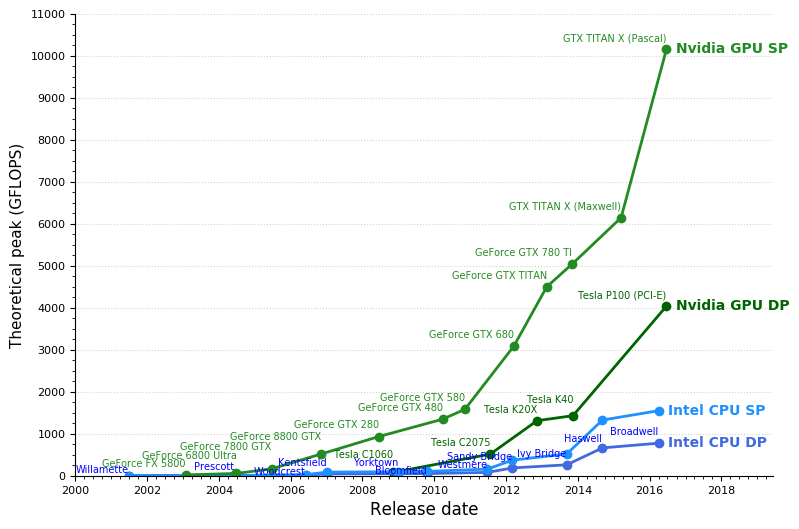
\includegraphics[width=.8\textwidth]{resources/graf.png}
	\caption{A graph showing the computational potential of CPUs and GPUs from 2000---2016 \cite{cpu-vs-gpu}}
	\label{potential}
\end{figure}

In this paper we will implement an autotuner for the programming language
Futhark \cite{futhark-home}. Futhark is a statically typed, data-parallel, and
purely functional array language. The aim of Futhark is to shift the burden of
writing efficient parallel code, from the programmer, to the compiler. The
burden referred to is that to write efficient GPU code, a deep understanding of
the hardware architecture, and the compiler is required. Not only does
languages such as CUDA and OpenCL require this, but even when this knowledge is
held it will result in non-portable code, since a lot of the optimizations made
will be specific to a certain GPU, or at least to a certain GPU architecture. 

\begin{figure}
\centering
\lstset{language=haskell}
\begin{lstlisting}
let dotprod [n] (xs: [n]f32) (ys: [n]f32): f32 =
reduce (+) 0f32 (map2 (*) xs ys)

let main [n][m][p] (xss: [n][m]f32) (yss: [m][p]f32): [n][p]f32 =
map (\xs -> map (dotprod xs) (transpose yss)) xss
\end{lstlisting}%
\captionof{lstlisting}{Matrix-matrix multiplication in Futhark \cite{ppopp}}
\label{IntromatmultFuthark}
\end{figure}
A Futhark program for matrix-matrix multiplication can be seen in listing
\ref{IntromatmultFuthark}, the syntax is similar to languages such as ML, and
Haskell. It is a good example of how Futhark differs from CUDA or OpenCL (we
would have liked to include an example of CUDA, but it was to long, so see
\ref{cuda-matmult} for a simpler version that only allows arrays of size
\textbf{FIX}). It's clear that if it's possible to achieve similar speeds 
with Futhark it would be very preferable over languages like CUDA.


To achieve this shift the Futhark compiler creates multiple semantically
equivalent versions of the code in a program, where each code version will
exploit a different amount of parallelism. These code versions are then to be
discriminated at runtime. To discriminate these code versions, Futhark asses
the amount of parallelism each function in the program contains, based on the
data being worked on. Put simply, if you have a matrix (\texttt{A}) of size $m
\times n$, and you execute a function (\texttt{inc}) incrementing each element,
then the parallel amount of \texttt{inc A} would be $m \times n$. Along with
these code versions, Futhark generates predicates that guard the code versions.
The aim is then to give a Futhark program parameters at runtime, and using the
guards, the knowledge of the hardware being execute on, along with the data
being worked on, it will select the best execution.

Adjusting these parameters to select the execution that will minimize the
running time is called tuning. The aim of this project is to automatize this
process, so that it doesn't have to be done by hand. This process is what we
call auto-tuning.

An analogy to tuning Futhark, is being a kid in a candy store. We have a bag
(parallel hardware, which will most commonly be a GPU), that is to be filled
with candy (parallelism in a program). We do not have a favorite type of candy
(the code versions being semantically equivalent), so we want to want to
efficiently pack the bag in order to get as much candy as possible. If we
overpack the bag, it will get to heavy (introducing overhead larger than gain)
and it will take longer to get the bag home, and if we underfill it, we will
obviously get less candy. Therefore we need to put a piece of candy in the bag
(a parallel function in the program), and then asses the next candy pieces
size, and the remaining capacity of the bag, and if the candy fits we put it in
(tuning the parameters). 
